\chapter{Results \& Discussions}

All the published papers declared results for their experiment where the controllers were tested either for CPU or RAM utilization. They performed tests using the OFNet tool to create a vast virtual network, send large packets to the server, and use OFCProbe or OFCBench to monitor the CPU and RAM utilization via the use of SMTP messages. However, instead of OFNet, multiple instances of CBench can also be used to send those packets.

In our experiment, we have used multiple instances of CBench and Mininet. We have also used Perf to read the system utilization information directly at the server.

After having our experiment, as illustrated in the workflow depicted in Fig. \ref{workflowexperiment}, the collected raw data is represented in a graphical format. We received and processed the system metrics such as CPU Utilization, Clock Speed, Instructions per Second, Branch mispredictions, and various level cache miss rates. These results are further discussed one by one.

\section{CPU Utilization}

\begin{figure}[!hbt]
    \centering
        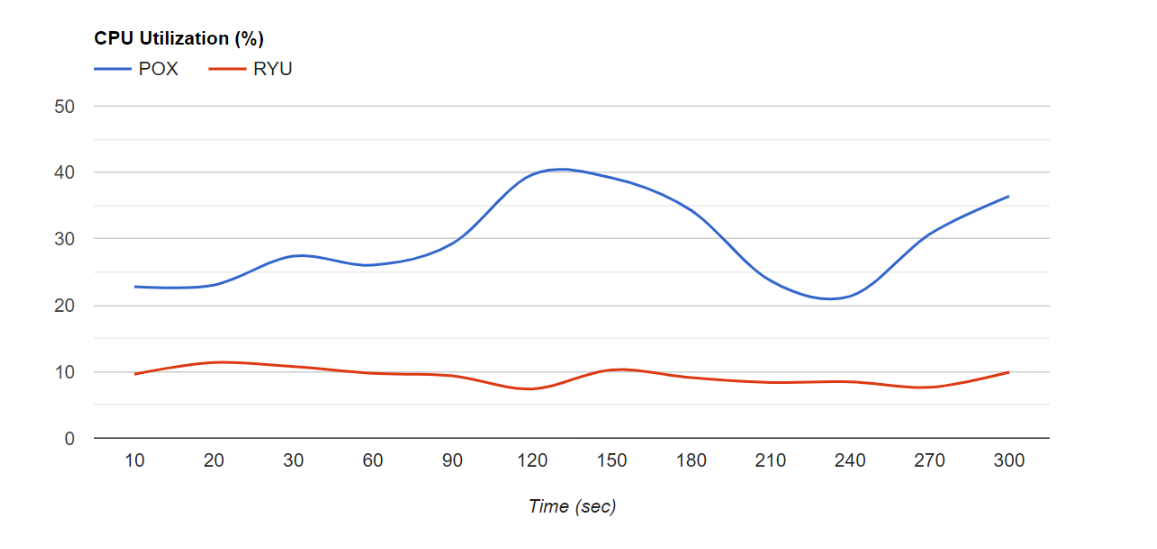
\includegraphics[width=\textwidth,keepaspectratio]{images/cpu_utilization.png}
       \caption{CPU Utilization}
        \label{CPUutilization}
\end{figure}

Usage of the CPU refers to the use of computing power by a process or the amount of work a CPU performs. Specific tasks require massive CPU time, while others require less because of non-CPU resource requirements. A method is said to be working better if, for the same number of tasks, it utilizes less CPU.

In our result, it shows that RYU continuously utilizes less CPU than POX, depicted in Fig. \ref{CPUutilization} However, it was not such as seen in Fig. \ref{figzhu2019sdn} taken from the paper published in 2018, that depicted for at least fewer time Pox too utilize the same as Ryu or even less CPU. \cite{zhu2019sdn}

\section{Instructions Per Second}

Instructions per Cycle (IPC), generally referred to as clock instructions, are one component of processor performance: the total number of instructions per clock cycle.

\begin{figure}[!hbt]
    \centering
        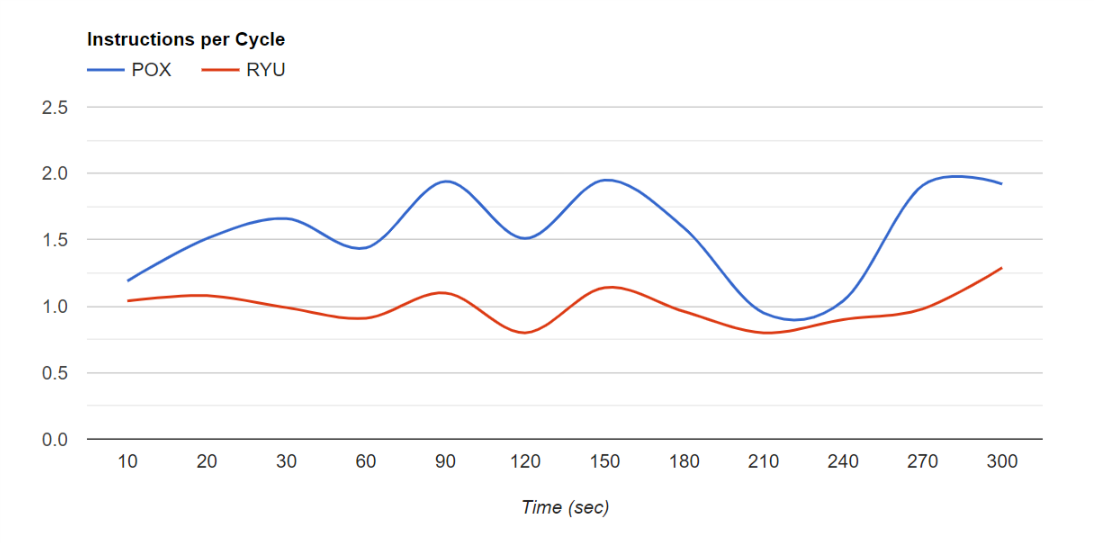
\includegraphics[width=\textwidth,keepaspectratio]{images/ipc.png}
       \caption{IPC}
        \label{ipc}
\end{figure}

With a specific processor, the number of instructions executed per clock is not a constant; it depends on how the individual program running communicates with the processor, and indeed the entire system, particularly the memory hierarchy. Nonetheless, certain CPU characteristics tend to contribute to designs with higher than average IPC values; the inclusion of several arithmetic logic units (an ALU is a CPU module capable of performing basic arithmetic and logical operations); and short pipelines. When evaluating various instruction sets, a simplified instruction set will contribute to a higher IPC number than applying a more complicated instruction set with the same chip technology; furthermore, with fewer instructions, the more complex instruction set may do more valuable work. 

The obtained result is depicted in Fig. \ref{ipc}. The efficient use of pipelining can be seen by both the controllers where both scored IPC values greater than 1. However, Pox, in contrast to Ryu, has better IPC.

\section{CPU Clock Speed}

CPU clock speed is calculated in Hertz — generally in gigahertz or GHz. Clock speed is a function of how many
clock cycles a Processor will execute per second. For example, a 1.8 GHz clock-rate CPU will execute 1,800,000,000 clock cycles per second. It looks so plain on the face. The more cycles a CPU can perform, the more it can do.

\begin{figure}[!hbt]
    \centering
        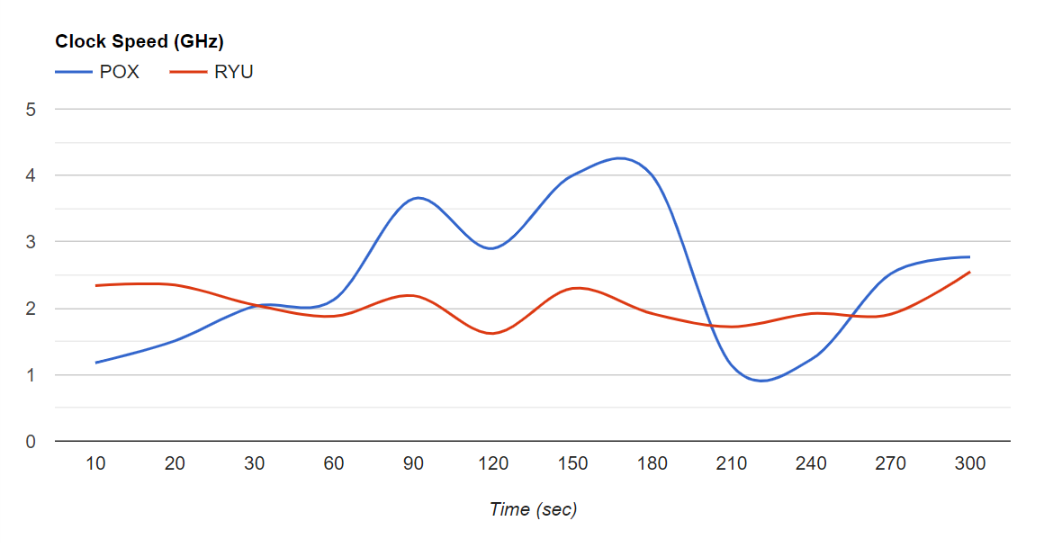
\includegraphics[width=\textwidth,keepaspectratio]{images/clock_speed.png}
       \caption{CPU Clock Speed}
        \label{clockspeed}
\end{figure}

On average both Ryu and Pox relatively has a similar clock speed of about a 2GHz. However, it is also seen from Fig. \ref{clockspeed} that Pox even touches a 4GHz score or more when required. Thus, confirming that the controller uses the Turbo Boost features provided by the system used for the experiment.

\section{L1 Cache Miss Rate}

In order to improve the performance of the cache, reducing the missing rate becomes one of the necessary steps. Decreasing access time to the cache also boosts its performance.

\begin{figure}[!hbt]
    \centering
        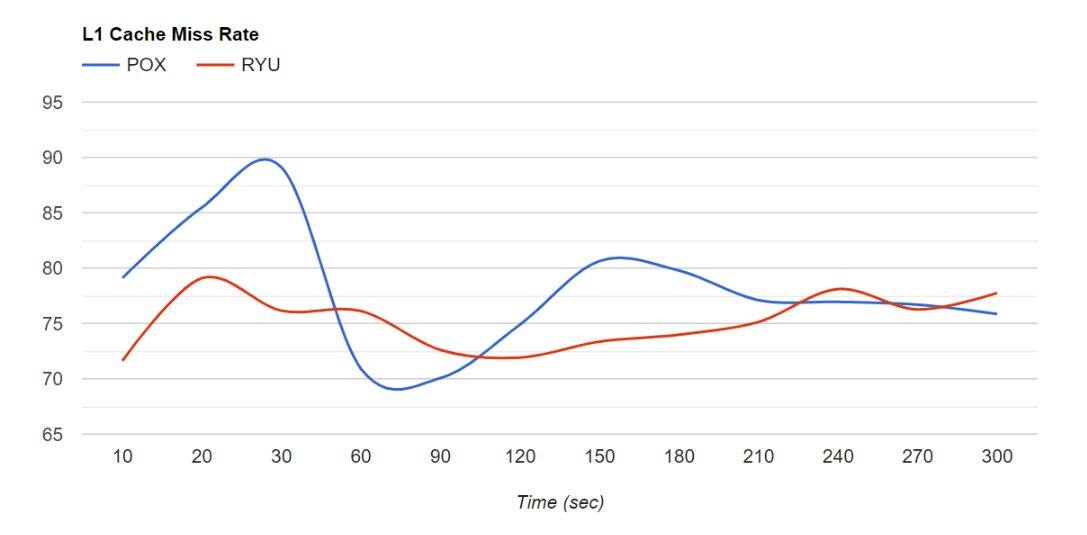
\includegraphics[width=\textwidth,keepaspectratio]{images/l1_miss_rate.png}
       \caption{L1 cache miss rate}
        \label{l1missrate}
\end{figure}

From the experiment as depicted in Fig. \ref{l1missrate}, it can be observed that on average, both Pox and Ryu has 80\% and 75\% of l1 miss rates respectively. This high miss rate is not enough for any real-time applications. However, during the initiation phase Pox even has the miss rate as high as 90\%.

\section{L2 Cache Miss Rate}

\begin{figure}[!hbt]
    \centering
        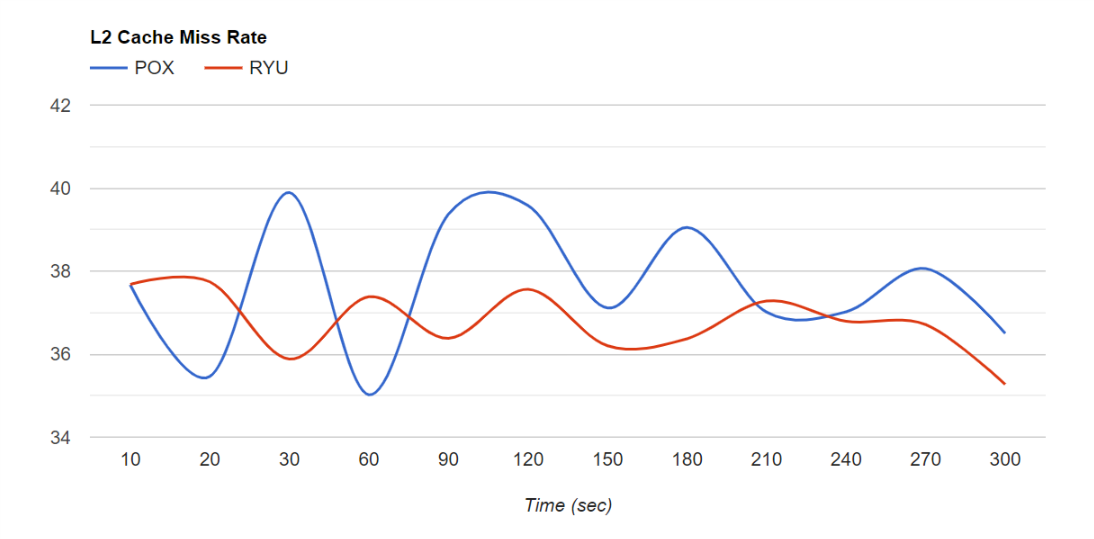
\includegraphics[width=\textwidth,keepaspectratio]{images/l2_miss_rate.png}
       \caption{L2 cache miss rate}
        \label{l2missrate}
\end{figure}

For level-2 cache, the miss rates are quite less than as compared to level-1 cache. The L2 miss rates for Ryu and Pox is observed to be below 40\%. However, about real-time applications that need to run 24*7 less than the observed.

\section{Branch Misprediction}

Branch Predictions are an architectural innovation that provides an alternative to conditional control transfers, enforced by computer commands, such as conditional branch, conditional call, tentative return and tables for branches. Predication operates by implementing instructions from both branch directions, enabling only specific instructions from the path taken to change architectural condition.

\begin{figure}[!hbt]
    \centering
        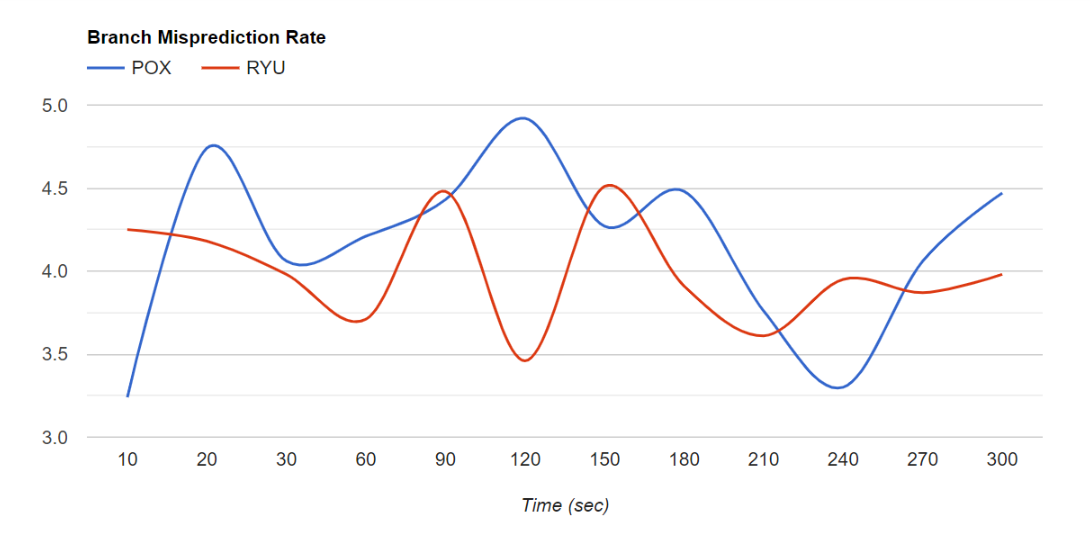
\includegraphics[width=\textwidth,keepaspectratio]{images/branch_mispredicted.png}
       \caption{Branch Misprediction Rate}
        \label{branchmisprediction}
\end{figure}

The branch predictor aims to boost flow inside the instruction pipeline. In several modern pipelined microprocessor architectures such as x86, branch predictors play a critical role in achieving highly effective performance. Predictor latency can also have
a profound impact on efficiency. Branch Misprediction Rate is the ratio that indicates the rate of mispredicted branches.

When there is a high rate of a branch misprediction, an optimization (minimization) problem is used where the
emphasis is on achieving the lowest possible miss rate, low power consumption and low resource complexity. 

As shown in Fig. \ref{branchmisprediction}, the result clearly shows, for both Ryu and Pox, this rate is quite low, i.e. below 5\%. Also, during initialization time (first 10 - 15 secs), Pox has this rate significantly lesser than Ryu. However, overall on average, Ryu has about 22\% fewer misprediction rates than Pox.